\documentclass{article}

\usepackage[swedish]{babel}
\usepackage[utf8]{inputenc}
\usepackage{amsmath}
\usepackage{hyperref}
\usepackage{underscore}
\usepackage{tikz}
\usepackage{tkz-euclide}
\usepackage{tikz-3dplot}
\usepackage{amsfonts}
\usepackage{mathtools}
\usepackage{enumitem}
\usepackage{blkarray}
\usepackage{xcolor}
\usetkzobj{all}

\DeclarePairedDelimiter \abs{\lvert}{\rvert}
\DeclarePairedDelimiter \norm{\lVert}{\rVert}

\hypersetup{
	pdfauthor={Adnan Avdagic},
	pdftitle={TATA69 Föreläsningar},
	colorlinks}

\begin{document}
\title{TATA69 Föreläsningar}
\author{Adnan Avdagic\\
	Linköpings Universitet\\
	\texttt{adnan@avdagic.net}}
\date{\today}
\maketitle

\newpage

\tableofcontents

\newpage
\noindent

\section{Föreläsning 2}
\subsection{Gränsvärden för flervarre}

\paragraph{Exempel 1} \flushleft
\begin{equation} \label{eq:1}
	f(x,y) = \frac{\sin(x^4+y^2)}{x^4+y^2} \text{, ej definderad i origo}
\end{equation}

Vad händer då (x,y) närmar sig (0,0)?

$$\lim_{x,y \rightarrow 0,0} \frac{\sin(x^4+y^2)}{x^4+y^2}$$

//sätt $t= \displaystyle x^4+y^2$, ${t \rightarrow 0}$ då ${(x,y) \rightarrow (0,0)}$// \newline
då fås \(\displaystyle \lim_{t \rightarrow 0} \frac{\sin t}{t} = 1,\) (standard gränsvärde) \newline

\paragraph{Exempel 2} \flushleft
\begin{equation} \label{eq:2}
	f(x,y) = \frac{x^3+xy}{x^2+y^2} \text{, ej definderad i origo}
\end{equation}

Gå mot origo via x-axeln (där $y=0$)
\[f(x,0) = \frac{x^3+0*x}{x^2+0^2} = \frac{x^3}{x^2} =  {x \rightarrow 0} \text{ då } {x \rightarrow 0}\]

Gå mot origo via y-axeln (där $x=0$)
\[f(0,y) = \frac{0^3+0*y}{0^2+y^2} = \frac{0}{y^2} =  {0 \rightarrow 0} \text{ då } {y \rightarrow 0}\]

Gå mot origo längs $y=x$
\[f(x,x) = \frac{x^3+x*x}{x^2+x^2} = {\frac{x+1}{2} \rightarrow \frac{1}{2}} \text{ då } {x \rightarrow 0}\]

Olika värden från olika riktningar \newline
Innanför varje liten cirkel kring origo har f värden nära 0 och nära $\frac{1}{2}$.
Vi säger därför att gränsvärde ej existerar. Se \ref{fig:1}

\begin{figure}[ht] 
\begin{tikzpicture}
   \tkzInit[xmax=5,ymax=5,xmin=-5,ymin=-5]
   \tkzAxeXY
   \draw[red,thick] (-5,0) -- (5,0);
   \draw[blue,thick] (0,-5) -- (0,5);
   \draw[green,thick] (-5,-2) -- (5,3);
   \node[above,red] at (-4,0) {\(f=x\)};
   \node[right,blue] at (0,5) {\(f=0\)};
   \node[left,green] at (3,3) {\(f=\frac{x+1}{2}\)};
   \tkzDefPoint(0,0){O}
   \tkzDefPoint(0.2,0.2){A}
   \tkzDrawCircle(O,A)
  \end{tikzpicture}
  \caption{Graf i 2D} \label{fig:1}
\end{figure}

\newpage
\paragraph{Definition}

Funktionen \(\bar{f}\) av typ \(\mathbb{R}^n \rightarrow \mathbb{R}^m\) har gränsvärdet \(\bar{b} \in \mathbb{R}^m\) då \(\bar{x} \rightarrow \bar{a} \in \mathbb{R}^n\) om \(\forall \epsilon >0 \quad \exists \delta >0\) så att \(|\bar{f}(x)-\bar{b}|<\epsilon\) om \(0<|\bar{x}-\bar{a}|<\delta\) och \(\bar{x}\in D_f\). 
Skrivs 
\[
\lim_{\bar{x} \rightarrow \bar{a}} \bar{f}(\bar{x})=\bar{b}
\]

\newpage
\paragraph{Exempel 3}
\begin{equation} \label{eq:3}
	f(x,y)=\frac{x^3}{x^2+y^2} \text{, ej definderad i origo}
\end{equation}

\[
\begin{split}
0 \leq \abs{f(x,y)} = \frac{\abs{x^3}}{x^2+y^2} = \abs{x}\frac{x^2}{x^2+y^2} \leq \abs{x} \rightarrow 0 \text{ då } (x,y) \rightarrow (0,0) \\
\Rightarrow f(x,y) \rightarrow (0,0) \text{ då } (x,y) \rightarrow (0,0)
\end{split}
\]

Vanliga räkneregler för gränsvärden (summa, produkt, instängning) gäller också för flervarregränsvärden
Undersökning/beräkning av gränsvärden

\begin{itemize}
\item Om test av värden längs olika riktningar eller olika kurvor ger olika resultat så saknas gränsvärde, se \eqref{eq:2}
\item Sådana test kan \underline{INTE} visa att gränsvärde existerar, andra metoder behövs, som \eqref{eq:1} eller \eqref{eq:3}, eller polära koordinater
\end{itemize}

\begin{figure}[ht] 
\begin{tikzpicture}
   \tkzInit[xmax=4,ymax=4,xmin=0,ymin=0]
   \tkzAxeXY
   \tkzDefPoint(3,3){P} \tkzDefPoint(0,0){O}
   \tkzDefPoint(3,0){a} \tkzDefPoint(0,3){b} \tkzDefPoint(1.5,0){c}
   \tkzDrawArc[color=red](O,c)(P)
   \tkzDrawPoints(P)
   \tkzDrawSegment[blue](O,P)
   \tkzDrawSegment[dashed](a,P)
   \tkzDrawSegment[dashed](b,P)
   \node[right,red] at (1.5,0.5) {$\varphi$};
   \node[above left,blue] at (1.5,1.5) {$\rho$};
   \node[above right] at (3,3) {(x,y)};
  \end{tikzpicture}
  \caption{Graf för polära koordinater} \label{fig:2}
\end{figure}

\[
	\def\arraystretch{1.1}
	\begin{blockarray}{r@{\;}l}
	\begin{block}{r@{\;}l\}}
		x & = \rho \cos(\varphi) \\[\jot]
		y & = \rho \sin(\varphi) \\[\jot]
	\end{block}
	\rho  & = \sqrt{x^2+y^2} \text{, } \rho > 0 \\ [\jot]
	\tan{\varphi} & = \frac{y}{x} \text{, } 0 \leq \varphi \leq 2\pi
	\end{blockarray}
\]
Viktigt för gränsvärden: \( (x,y) \rightarrow (0,0) \iff \rho \rightarrow 0 \)

\newpage

\paragraph{Exempel \eqref{eq:3} med polära koordianter}

\[
	\lim_{(x,y) \rightarrow (0,0)} \frac{x^3}{x^2+y^2} \overset{\mathrm{pol.koord}}{=} \lim_{(\rho \rightarrow 0} \frac{\rho^3\cos^3(\varphi)}{\rho^2} = \lim_{\rho \rightarrow 0} \overbrace{\rho}^{\rightarrow\infty}\underbrace{\cos^3(\varphi)}_\text{begränsad} = 0
\]

\paragraph{Exempel \eqref{eq:2} med polära koordianter}

\[
\begin{split}
\lim_{(x,y) \rightarrow 0} \frac{x^3+xy}{x^2+y^2} \overset{\mathrm{pol.koord}}{=} \lim_{\rho \rightarrow 0} \frac{\rho^3 \cos^3(\varphi) + \rho^2 \cos(\varphi) \sin(\varphi)}{\rho^2} = \\
=\lim_{\rho \rightarrow 0} (\overbrace{\rho \cos^3(\varphi)}^{\rightarrow 0}+\underbrace{\cos(\varphi) \sin(\varphi)}_\text{vinkelberoende}) \Rightarrow \text{gränsvärde exiterar ej}
\end{split}
\]

\paragraph{Oändlighet i envarre och flervarre}
\subparagraph*{Envarre}
x kan gå mot $\pm\infty$
\subparagraph*{Flervarre}
bara en $\infty$ nämligen $\abs{\bar{x}} \rightarrow \infty$
\subparagraph*{2D polära}
$\abs{\bar{x}} \rightarrow \infty \iff \rho \rightarrow \infty$
\paragraph{Definition}
\[
	\bar{f}(\bar{x}) \rightarrow \bar{b} \text{ då } \abs{\bar{x}} \rightarrow \infty \text{ om } \forall \epsilon > 0 \quad \exists \omega \text{ så att } \abs{\bar{f}(\bar{x}) - \bar{b}} < \epsilon \text{ om } \abs{\bar{x}} > \omega
\]

\newpage
\paragraph{Exempel 4}

\begin{equation} \label{eq:4}
	\lim_{(x,y) \rightarrow \infty} \frac{y}{x^2+y^2} \overset{\mathrm{pol.koord}}{=} \lim_{\rho \rightarrow \infty} \frac{\rho \sin(\varphi)}{\rho^2} = \lim_{\rho \rightarrow \infty} \overbrace{\frac{1}{\rho}}^{\rightarrow 0} \underbrace{\sin(\varphi)}_\text{Begränsad} = 0
\end{equation}

\underline{OBS!} 2-variablefunktioner som uttryckta i polärakoordinater inte beror på $\varphi$ har rotationssymetriska grafer kring z-axeln

\begin{figure}[ht]
\usetikzlibrary{3d}
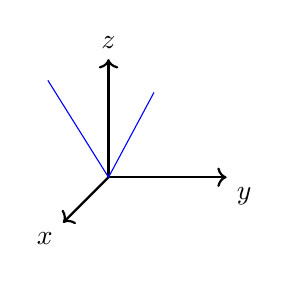
\begin{tikzpicture}
\draw[thick,->] (0,0,0) -- (0,0,1.5) node[anchor=north east]{$x$};
\draw[thick,->] (0,0,0) -- (1.5,0,0) node[anchor=north west]{$y$};
\draw[thick,->] (0,0,0) -- (0,1.5,0) node[anchor=south]{$z$};
\foreach \p in {1,...,360} {
	\draw[red] ({sin(45)*sin(\p)},{cos(45)},{sin(45)*cos(\p)}) -- ({sin(45)*sin(\p)},{cos(45)},{sin(45)*cos(\p)});
}
\draw[blue] (0,0,0) -- (0,2,2);
\draw[blue] (0,0,0) -- (0,0.5,-1.5);
\end{tikzpicture}
\caption{Exempel på rotationssymmetri} \label{fig:3}
\end{figure}

\(
z = \sqrt{x^2+y^2} = \rho
\)

\subsubsection{3-variabler mot origo}
\paragraph{Exempel 5}

\begin{equation}
	\lim_{(x,y,z) \rightarrow (0,0,0)} \frac{xyz}{x^2+y^2+2z^2} = \text{ ???}
\end{equation}

\[
	0 \leq \abs{\frac{xyz}{x^2+y^2+2z^2}} = \frac{\abs{x}\abs{y}\abs{z}}{x^2+y^2+2z^2} \leq \frac{\abs{x}\abs{y}\abs{z}}{x^2+y^2+z^2} \leq 
\]

\[
	// 
	\def\arraystretch{1.1}
	\begin{blockarray}{r@{\;}l}
	\abs{x} \leq \sqrt{x^2+y^2+z^2} \\ [\jot]
	\abs{y} \leq \sqrt{x^2+y^2+z^2} \\ [\jot]
	\abs{z} \leq \sqrt{x^2+y^2+z^2}
	\end{blockarray}
	//
\]

\[
	\leq \frac{\sqrt{x^2+y^2+z^2}}{x^2+y^2+z^2} = \sqrt{x^2+y^2+z^2} \rightarrow 0 \text{ då } (x,y,z) \rightarrow (0,0,0)
\]

\newpage
\subsection{Rymdpolärakoordianter}

\begin{figure}[ht]
\usetikzlibrary{3d}
\begin{tikzpicture}
\draw[thick,->] (0,0,0) -- (0,0,5) node[anchor=north east]{$x$};
\draw[thick,->] (0,0,0) -- (5,0,0) node[anchor=north west]{$y$};
\draw[thick,->] (0,0,0) -- (0,5,0) node[anchor=south]{$z$};
\draw[dashed]
	(0,4,0) --
	(4,4,4) coordinate (p) --
	(4,0,4) coordinate (q);
\draw[thick,red]
	(0,0,0) coordinate (o)-- (q);
\draw[dashed] 
	(0,0,4) coordinate (x) -- (q) -- (4,0,0);
\draw[thick,blue] (o) -- (p);
\draw[green] let
	\p0 = (o),
	\p1 = (0,0,2),
	\p2 = (2,0,2),
	\n1 = {atan2(\p1)},
    \n2 = {\n1 + 103},
    \n3 = {1cm},
    \n4 = {(\n1 + \n2) / 2}
  in (o) +(\n1:\n3) arc[radius = \n3, start angle = \n1, end angle = \n2];
\draw[purple] let
	\p0 = (o),
	\p1 = (0,0,2),
	\p2 = (2,0,2),
	\n1 = {atan2(2,0)},
    \n2 = {atan2(2,2)},
    \n3 = {1cm},
    \n4 = {(\n1 + \n2) / 2}
  in (o) +(\n1:\n3) arc[radius = \n3, start angle = \n1, end angle = \n2];
\node[fill,circle,inner sep=1.5pt,label={above right:$(x,y,z)$}] at (p) {};
\node[left,blue] at (2,2,2) {$r$};
\node[right,red] at (1,0,1) {$r\sin(\theta)$};
\node[above,green] at (1,0,2.5) {$\varphi$};
\node[above left,purple] at (0.7,1,0) {$\theta$};
\end{tikzpicture}
\caption{Rymdpolära koordinater} \label{fig:4}
\end{figure}

\[
	\def\arraystretch{1.1}
	\begin{blockarray}{r@{\;}l}
	\begin{block}{r@{\;}l\}}
		x & = r \sin(\theta) \cos(\varphi) \\[\jot]
		y & = r \sin(\theta) \sin(\varphi) \\[\jot]
		z & = r \cos(\theta) \\[\jot]
	\end{block}
	r & = \sqrt{x^2+y^2+z^2} \text{, } r > 0 \\[\jot]
	0 & \leq \varphi \leq 2\pi \\[\jot]
	0 & \leq \theta \leq \pi \\[\jot]
	r & \sin(\theta) = \rho
	\end{blockarray}
\]

\newpage
\begin{appendix}
	\listoffigures
	\listoftables
\end{appendix}

\end{document}